\section{Appendix}
\label{app}

\subsection{Constitutional Artifacts}
\label{app:constArts}

\subsubsection{\mini}
\label{app:devRepo}
Access \mini at \href{https://minitwit.online/}{https://minitwit.online/}.

\subsubsection{Development Repository}
\label{app:devRepo}
\href{https://github.com/Akongstad/DevOps-group-p}{https://github.com/Akongstad/DevOps-group-p} Repository used for development, issue tracking, and projects

\subsubsection{Operations Repository}
\label{app:opsRepo}
\href{https://github.com/mikaeleythor/itu-minitwit-ops/tree/master}{https://github.com/mikaeleythor/itu-minitwit-ops/tree/master}
Repository used for deploying to production.

\subsubsection{Monitoring}
\label{app:monitoring}
Access the \mini monitoring dashboard: \href{https://minitwit.online/monitor}{https://minitwit.online/monitor}
\begin {figure}[H]
    \centering
    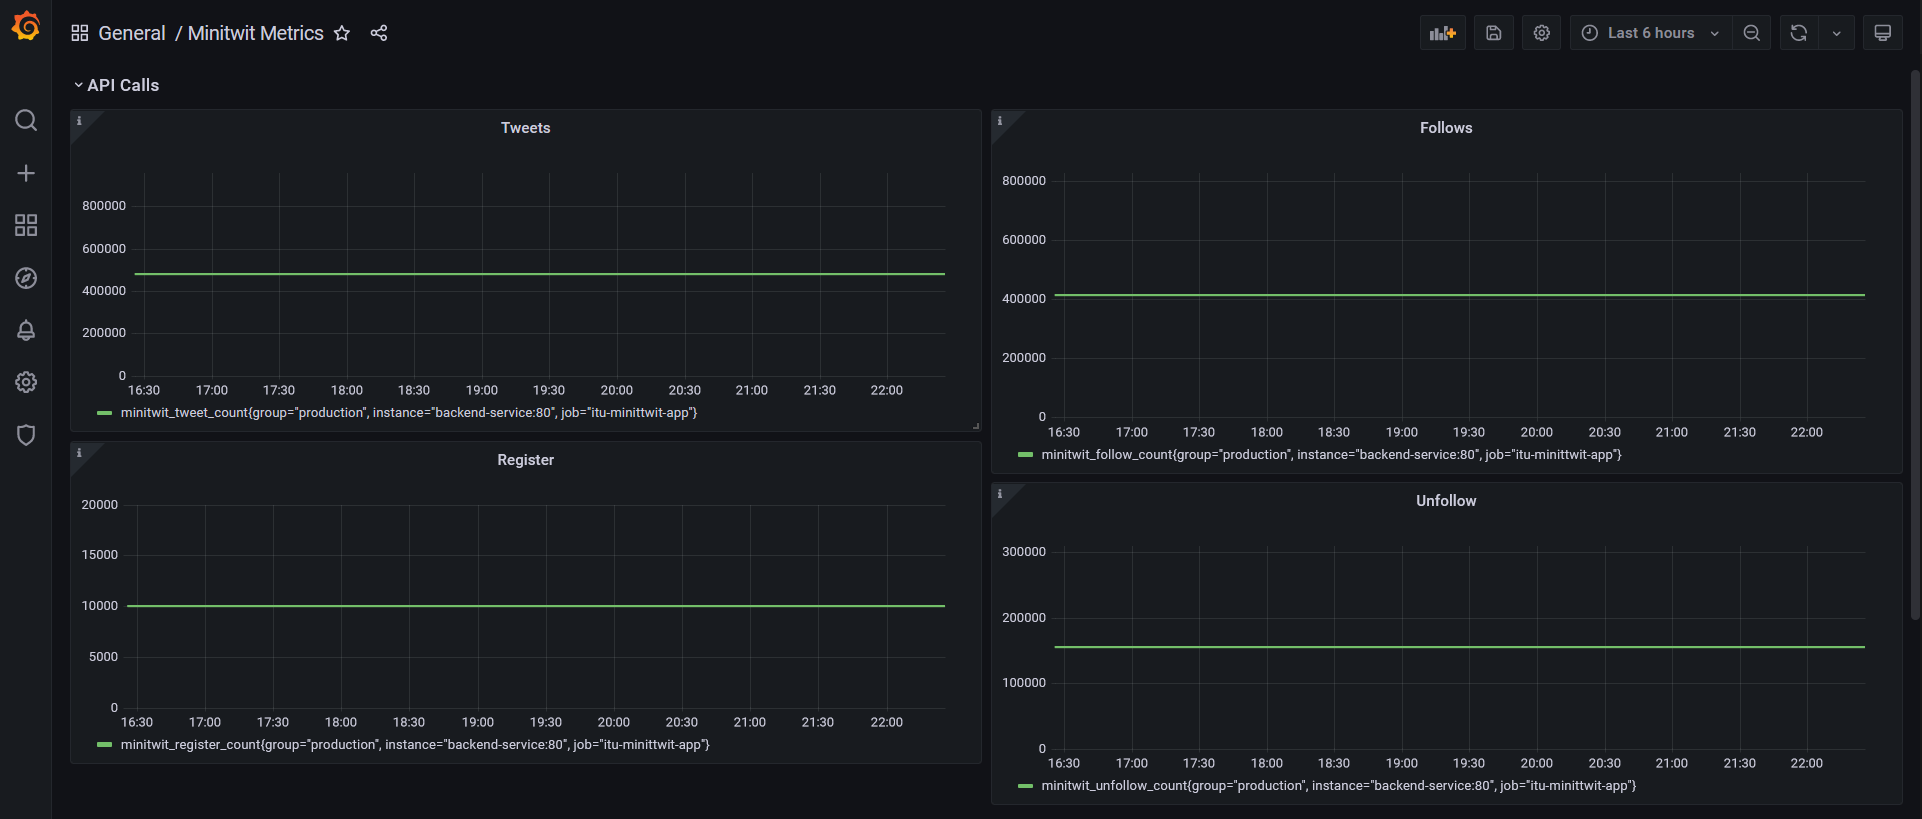
\includegraphics[scale=0.30]{images/monitoring/monitoring1.PNG}
    \caption{Monitoring Dashboard from  Grafana}
    \label{fig:simMonitor}
\end{figure}
\begin {figure}[H]
    \centering
    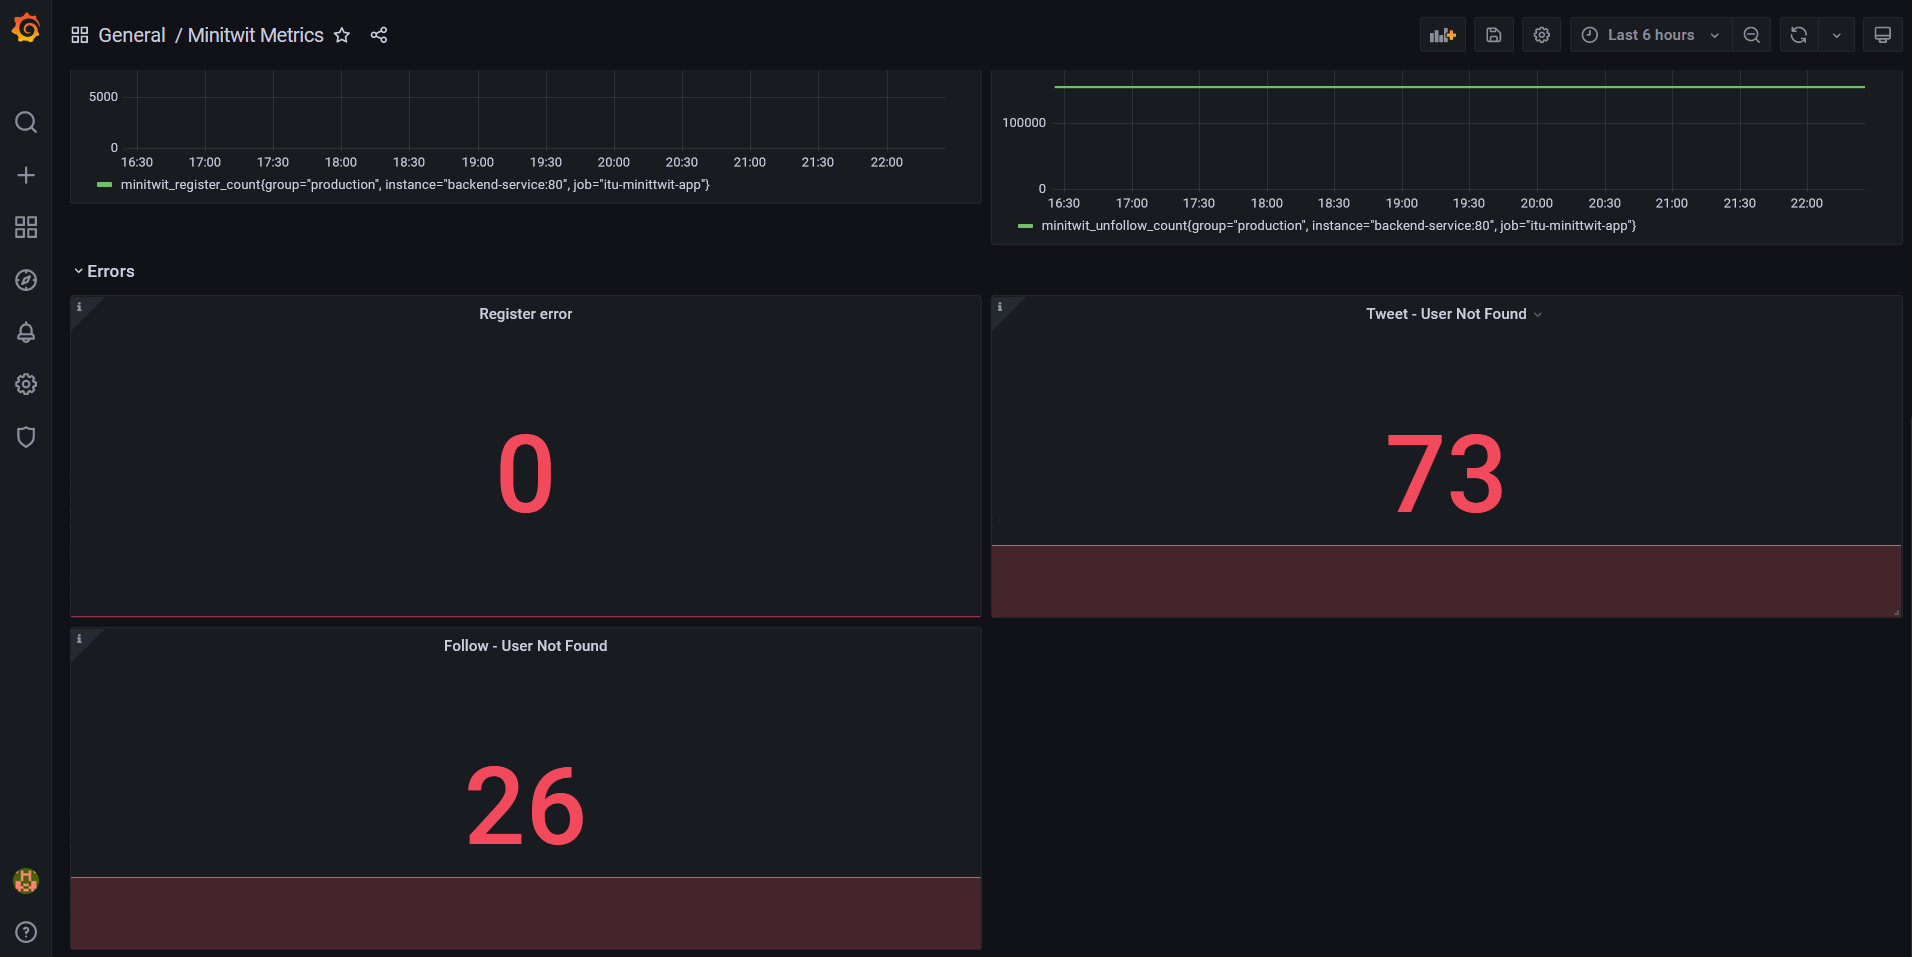
\includegraphics[scale=0.30]{images/monitoring/monitoring2.PNG}
    \caption{Monitoring Dashboard from  Grafana}
    \label{fig:simMonitor}
\end{figure}

\begin {figure}[H]
    \centering
    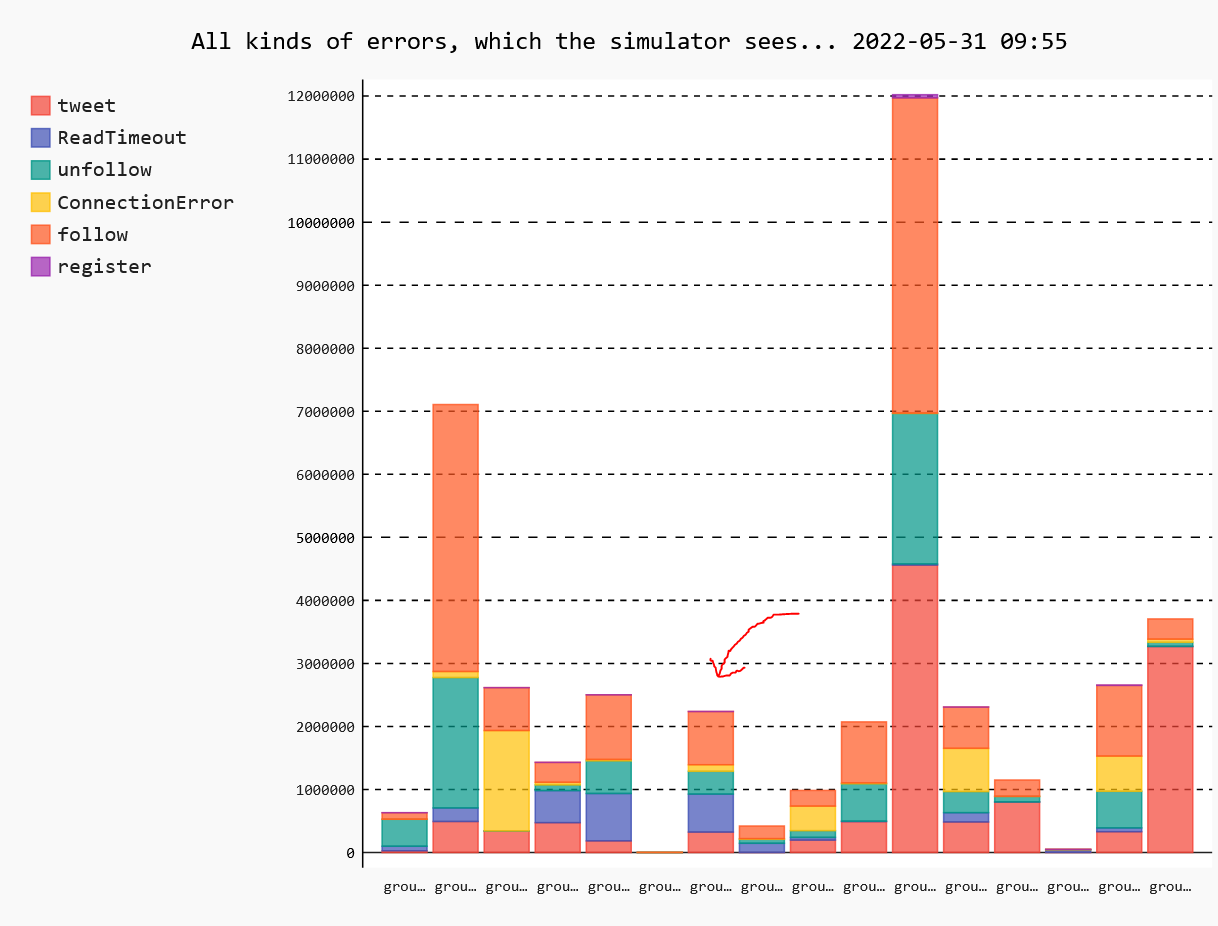
\includegraphics[scale=0.42]{images/monitoring/SimulatorMonitor.PNG}
    \caption{Monitoring Dashboard from the simulator}
    \label{fig:simMonitor}
\end{figure}



\subsection{Security Assessment}
\label{app:secAss}
\href{https://github.com/Akongstad/DevOps-group-p/blob/main/SECURITY.md}{https://github.com/Akongstad/DevOps-group-p/blob/main/SECURITY.md}

\subsubsection{Tests}
\label{app:testSuite}
\begin {figure}[H]
    \centering
    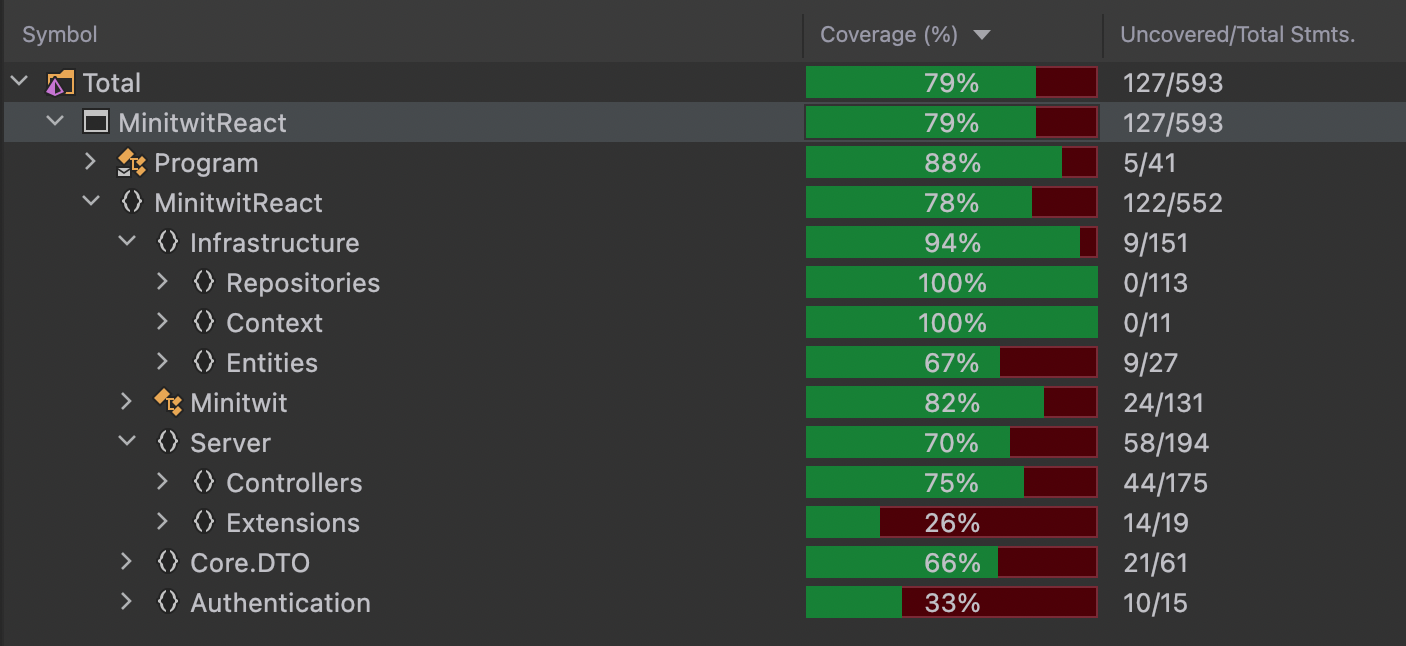
\includegraphics[scale=0.42]{images/testCoverage.png}
    \caption{Test coverage backend 31/05/22. (Generated code and main excluded)}
    \label{fig:testCov}
\end{figure}

\subsection{Code analysis dashboards}
\label{app:codeAnal}

\subsubsection{sonarcloud}
\label{app:codeAnalSonar}
\href{https://sonarcloud.io/project/overview?id=Akongstad_DevOps-group-p}{https://sonarcloud.io/project/overview?id=Akongstad\_DevOps-group-p}

\begin {figure}[H]
    \centering
    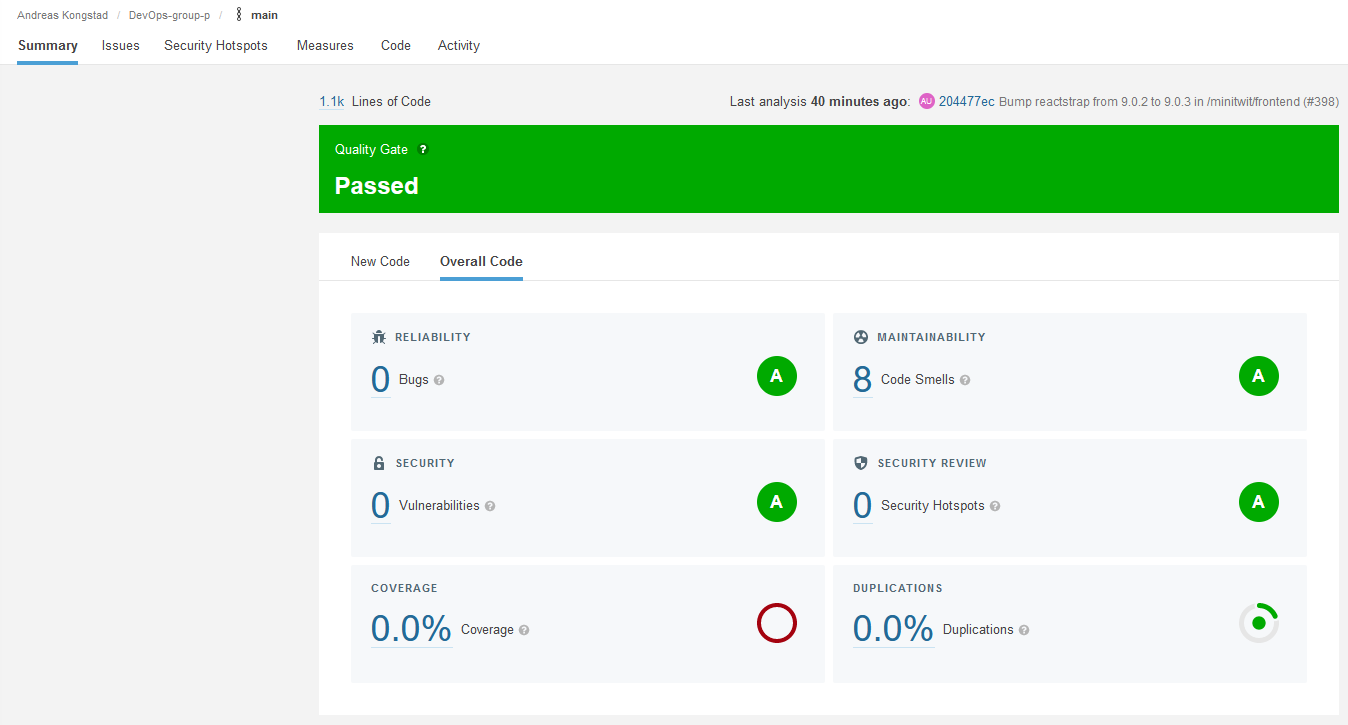
\includegraphics[scale=0.42]{images/analysis_tools/Sonar cloud backend.PNG}
    \caption{Sonarcloud maintainability scores 31/05/22}
    \label{fig:cloudMaintainability}
\end{figure}

\begin {figure}[H]
    \centering
    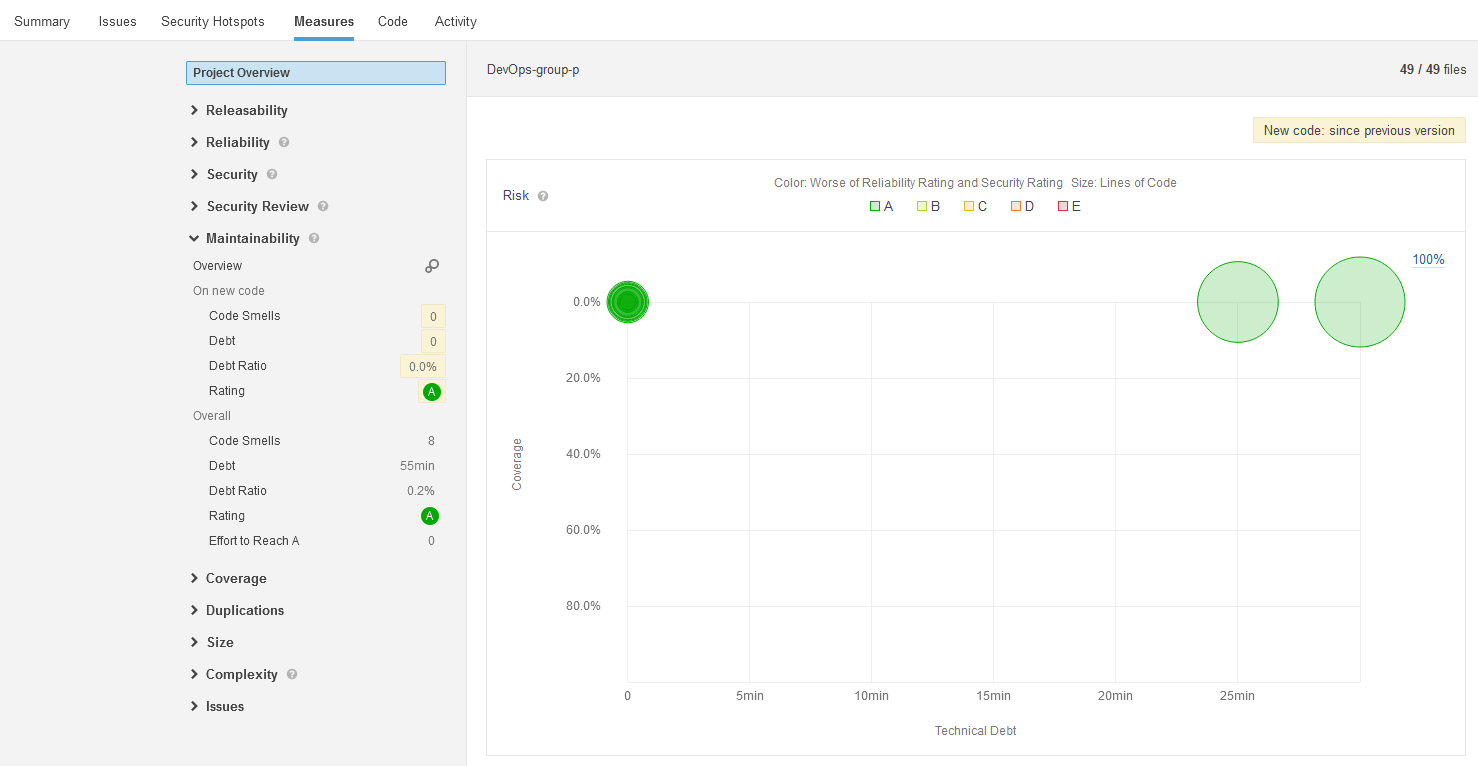
\includegraphics[scale=0.37]{images/analysis_tools/analys debt.PNG}
    \caption{Sonarcloud maintainability scores 30/05/22}
    \label{fig:cloudMaintainability}
\end{figure}

\begin {figure}[H]
    \centering
    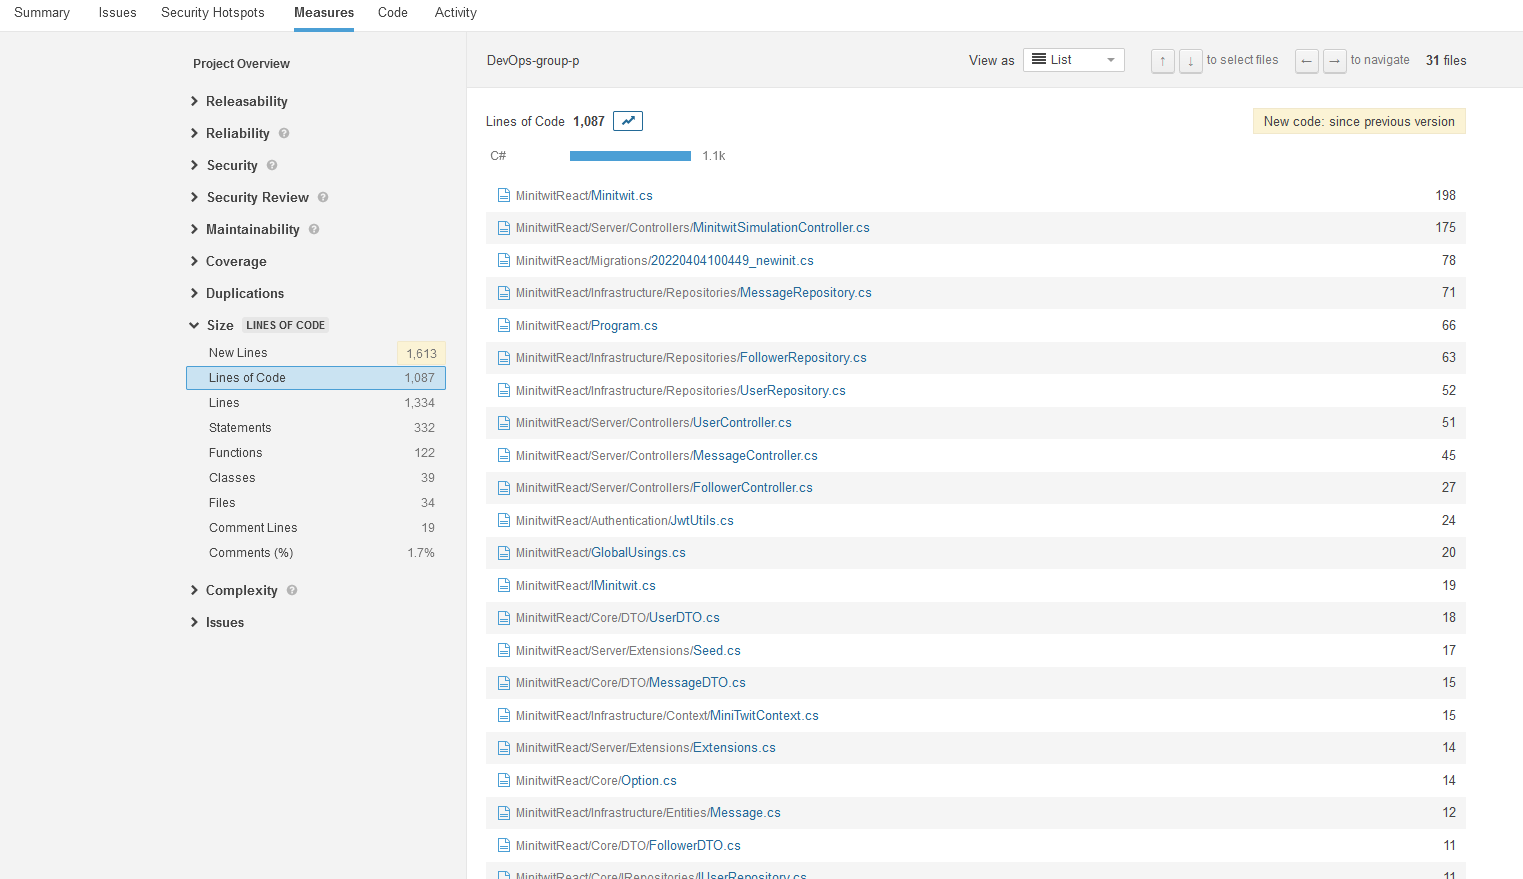
\includegraphics[scale=0.39]{images/analysis_tools/SonarCloudCsharp.PNG}
    \caption{Sonarcloud language distribution 31/05/22}
    \label{fig:cloudLangDis}
\end{figure}

\subsubsection{Code Climate}
\label{app:codeClimate}
\href{https://codeclimate.com/github/Akongstad/DevOps-group-p}{https://codeclimate.com/github/Akongstad/DevOps-group-p}

\begin {figure}[H]
    \centering
    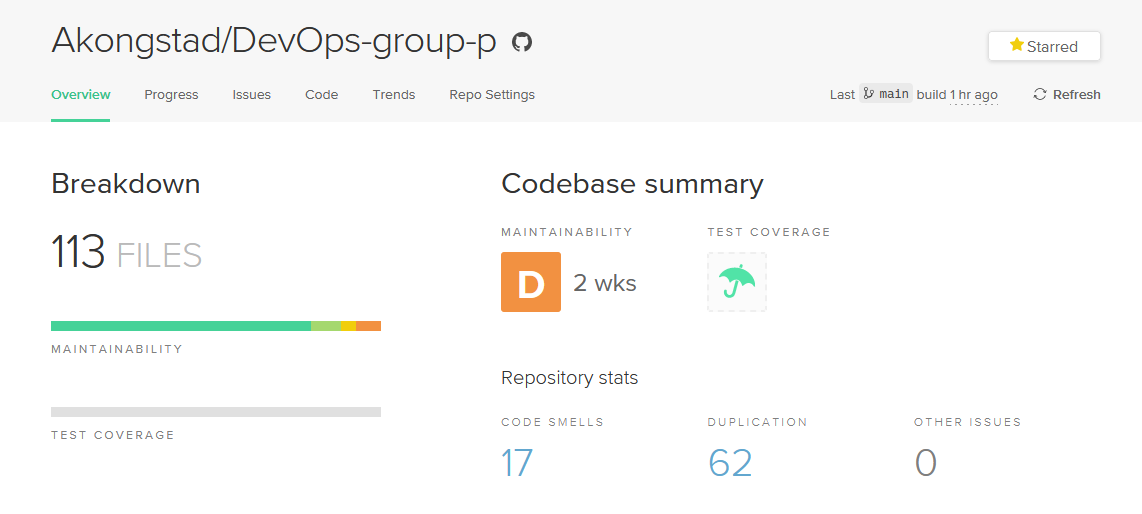
\includegraphics[scale=0.50]{images/analysis_tools/codeClimateDash.PNG}
    \caption{Code Climate repository status 31/05/22}
    \label{fig:codeClimateDash}
\end{figure}

\begin {figure}[H]
    \centering
    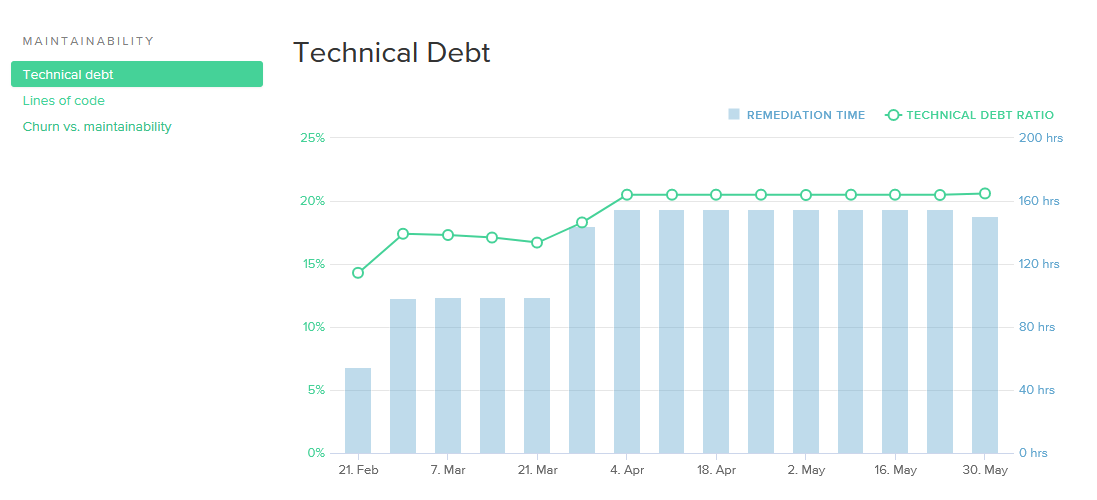
\includegraphics[scale=0.50]{images/analysis_tools/codeClimateTechDebt.PNG}
    \caption{Code Climate technical depth progression graph 31/05/22}
    \label{fig:codeClimateDepth}
\end{figure}

\begin {figure}[H]
    \centering
    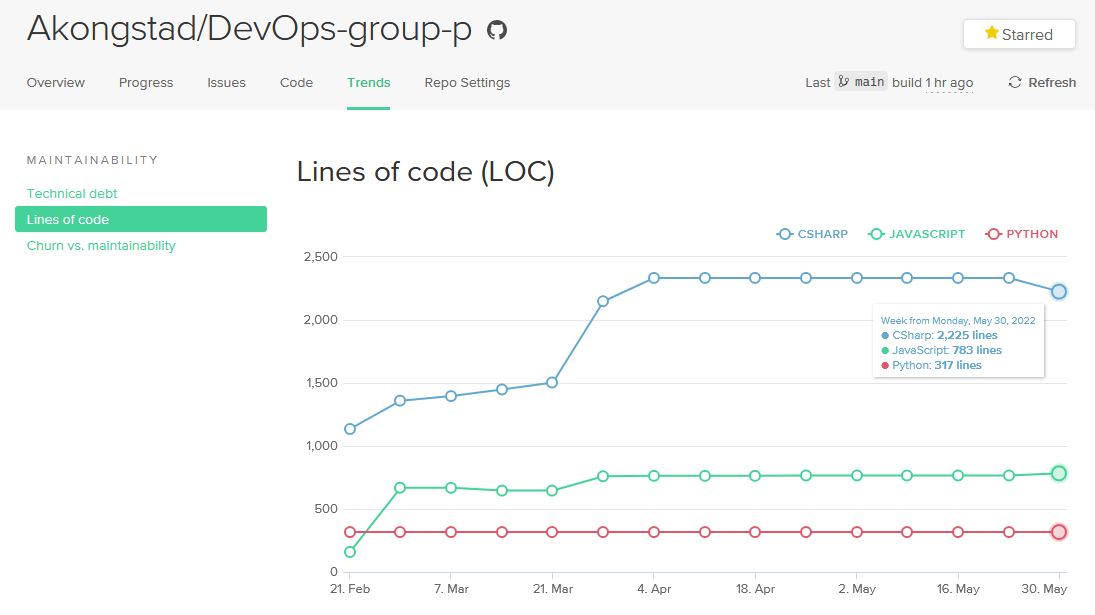
\includegraphics[scale=0.50]{images/analysis_tools/CodeClimateTrendsCode.PNG}
    \caption{Code Climate language distribution graph 31/05/22}
    \label{fig:codeClimateLangDis}
\end{figure}

\subsubsection{Better Code Hub}
\label{app:codeAnalHub}
\href{https://bettercodehub.com/results/Akongstad/DevOps-group-p}{https://bettercodehub.com/results/Akongstad/DevOps-group-p}

\begin {figure}[H]
    \centering
    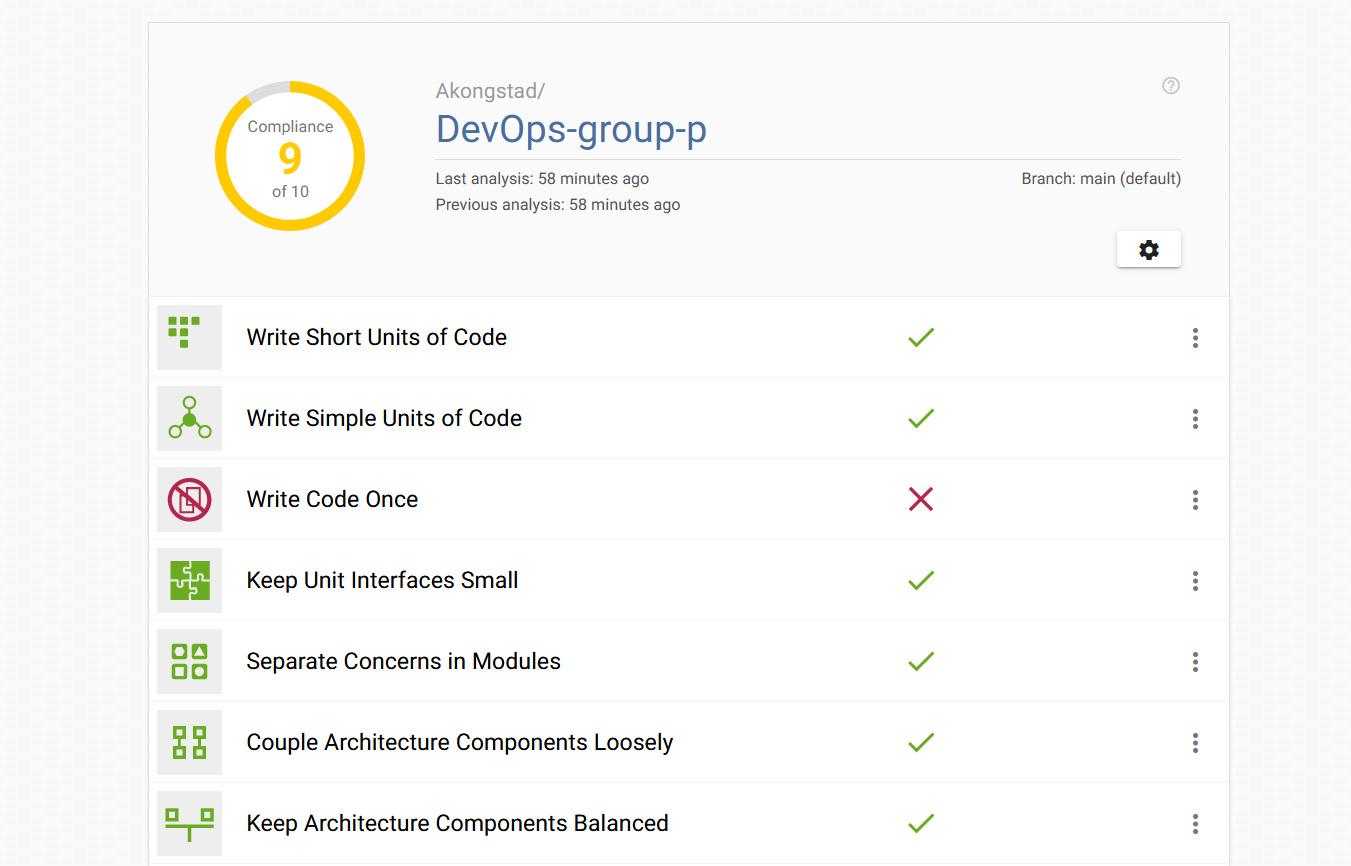
\includegraphics[scale=0.45]{images/analysis_tools/analysis 9of10.PNG}
    \caption{Better Code Hub repository status 30/05/22}
    \label{fig:hubStatus}
\end{figure}


\subsubsection{DeepScan}
\label{app:codeAnalDeep}
\href{https://deepscan.io/dashboard/\#view=project\&tid=17220\&pid=20572\&bid=562975}{https://deepscan.io/dashboard/\#view=project\&tid=17220\&pid=20572\&bid=562975}
\begin {figure}[H]
    \centering
    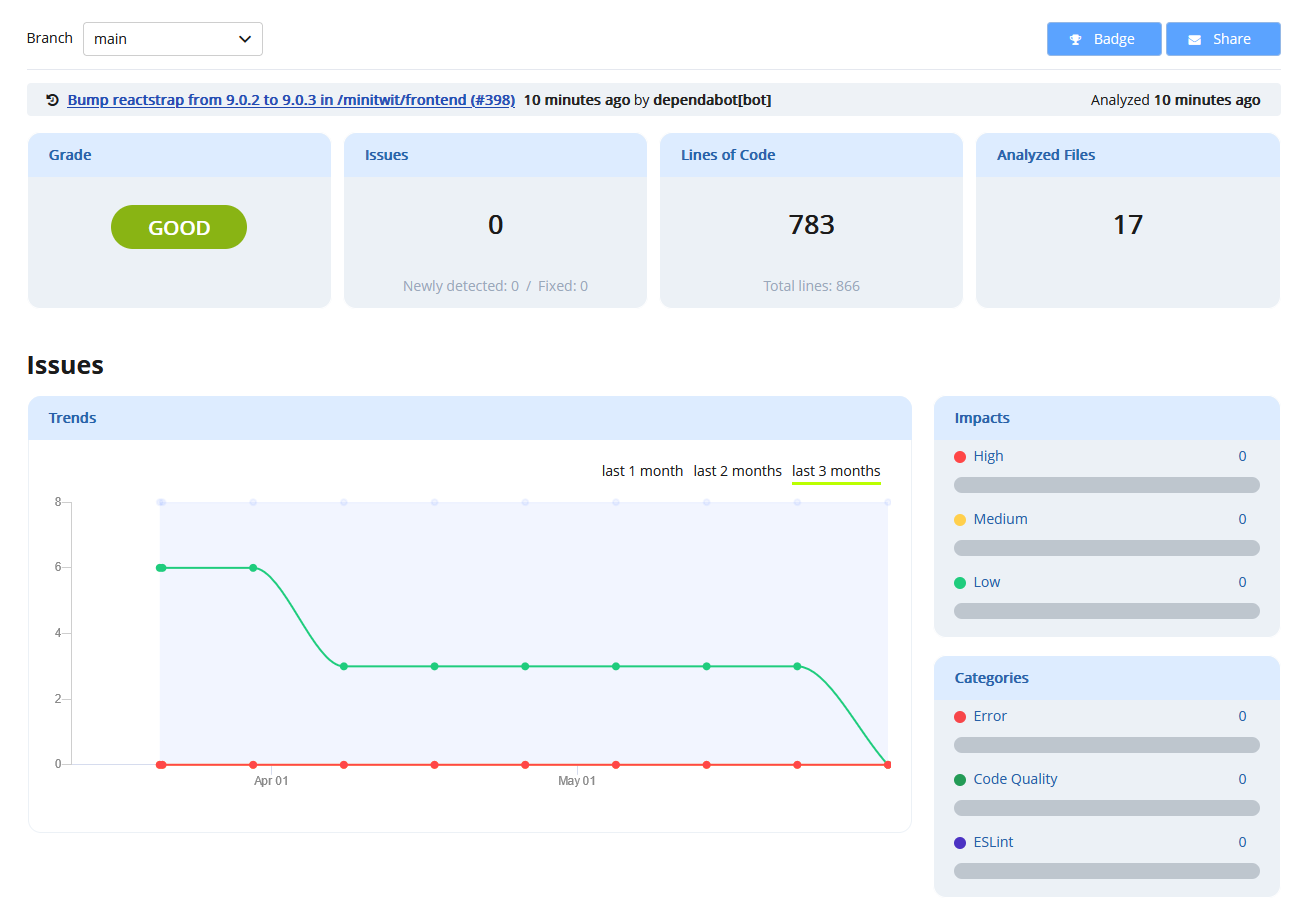
\includegraphics[scale=0.40]{images/analysis_tools/deepscan.PNG}
    \caption{DeepScan dashboard 31/05/22}
    \label{fig:deepscan}
\end{figure}

\subsubsection{snyk}
\label{app:codeAnalSnyk}
\href{https://app.snyk.io/org/akongstad}{https://app.snyk.io/org/akongstad}
\begin {figure}[H]
    \centering
    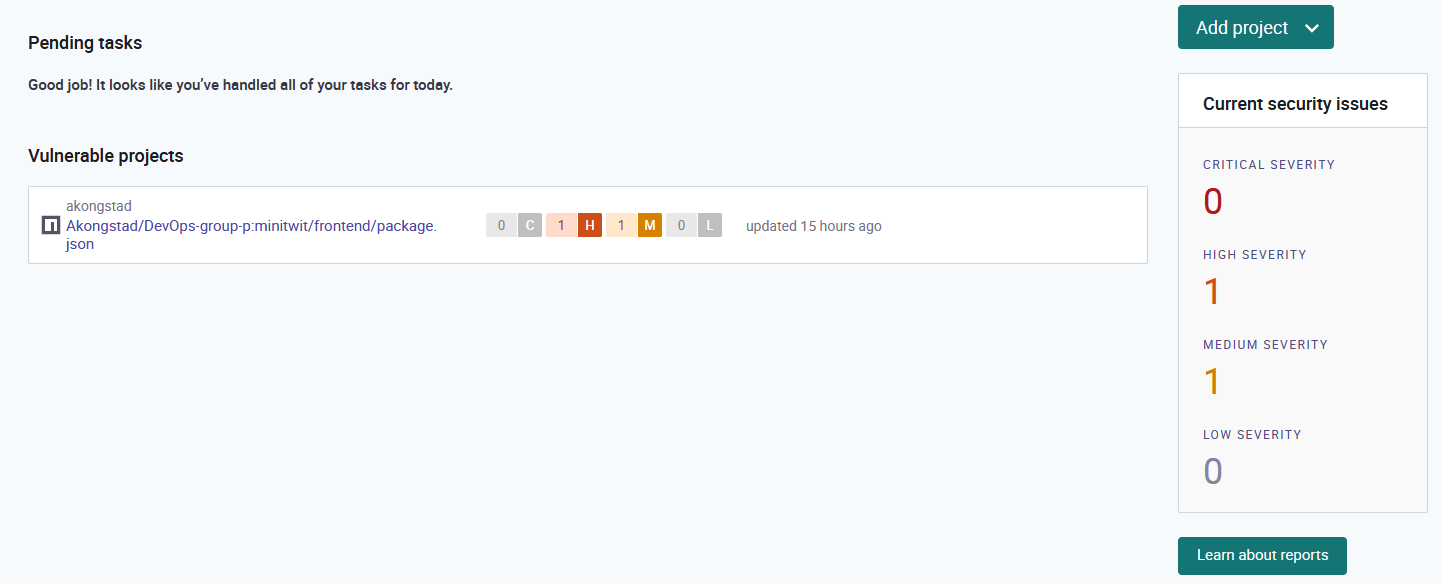
\includegraphics[scale=0.40]{images/analysis_tools/snykDashboard.PNG}
    \caption{Snyk Dashboard 31/05/2022}
    \label{fig:snykAlert}
\end{figure}

\begin {figure}[H]
    \centering
    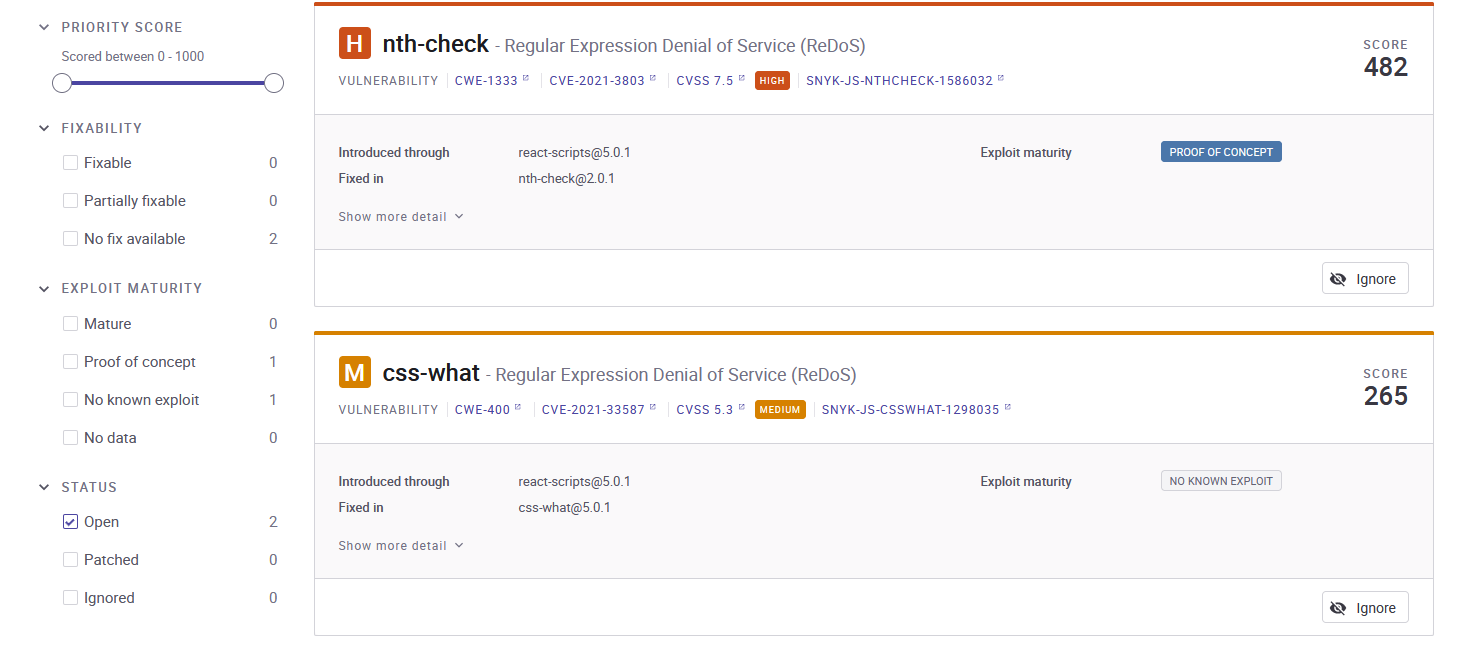
\includegraphics[scale=0.40]{images/analysis_tools/alertSnyk.PNG}
    \caption{Snyk scan alert 31/05/2022}
    \label{fig:snykAlert}
\end{figure}

\subsubsection{Github - Dependabot}
\label{app:codeAnalDependabot}
\href{https://github.com/Akongstad/DevOps-group-p/security/dependabot}{https://github.com/Akongstad/DevOps-group-p/security/dependabot}
\begin {figure}[H]
    \centering
    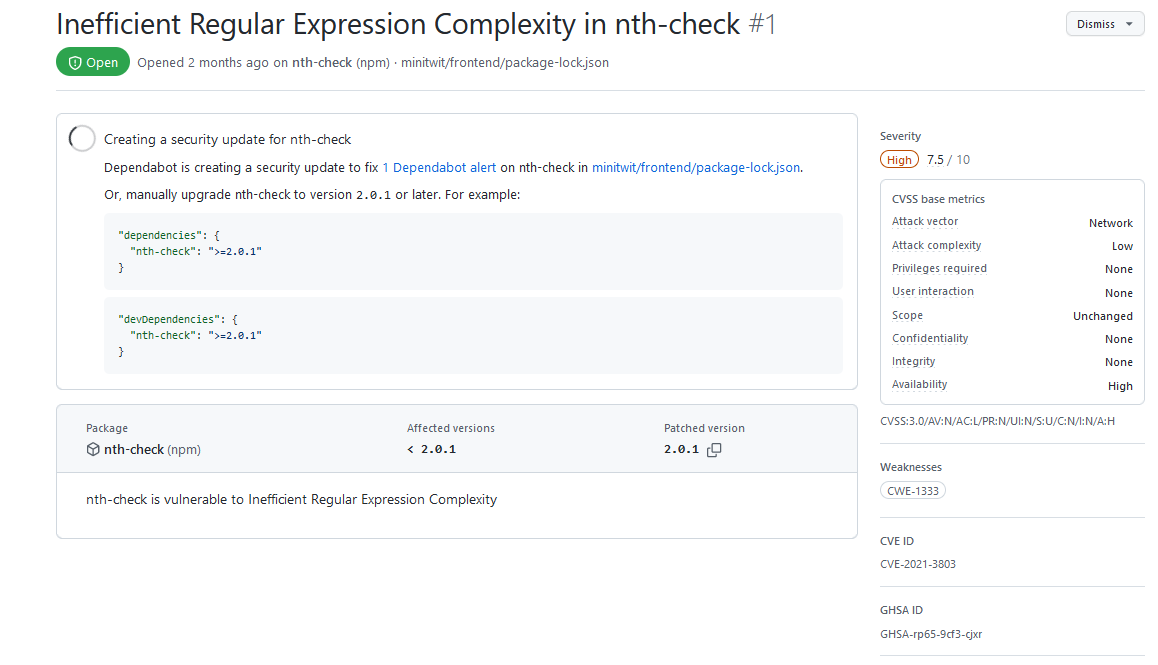
\includegraphics[scale=0.50]{images/analysis_tools/alertDependabot.PNG}
    \caption{Dependabot scan results 31/05/2022}
    \label{fig:dependabot}
\end{figure}

\subsubsection{Github - Code scanning tools}
\label{app:codeAnalQl}
\href{https://github.com/Akongstad/DevOps-group-p/security/code-scanning}{https://github.com/Akongstad/DevOps-group-p/security/code-scanning}

\begin {figure}[H]
    \centering
    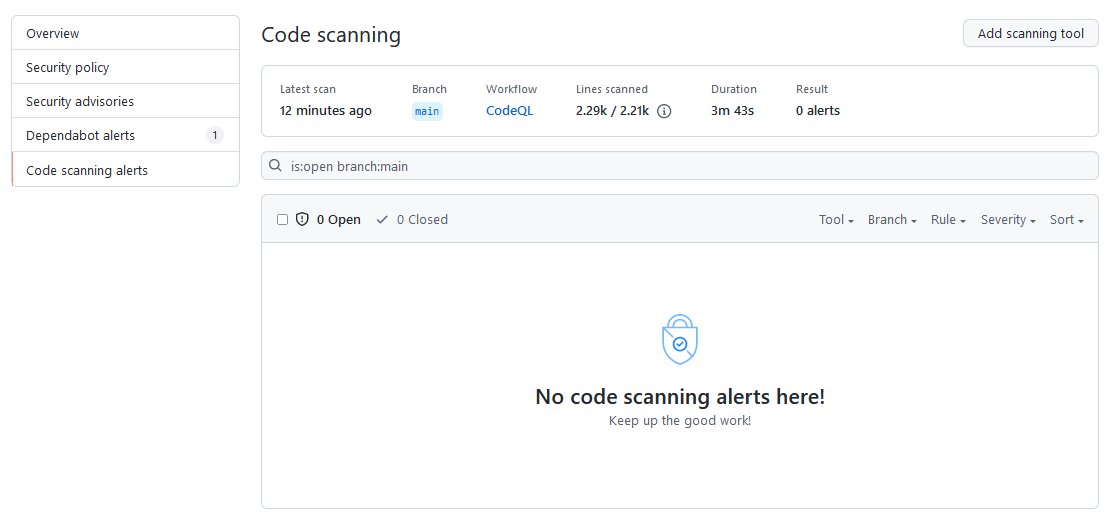
\includegraphics[scale=0.50]{images/analysis_tools/CodeQlScan.PNG}
    \caption{CodeQl scan results 31/05/2022}
    \label{fig:codeql}
\end{figure}

\subsection{Dependencies}
\label{app:dependencies}
\begin{enumerate}
    \item \textbf{Containerization} - Includes:
    \begin{itemize}
        \item \textbf{Docker} - Containerization platform.
        \item \textbf{Docker-Compose} - Running multiple containers in development.
        \item \textbf{Docker Hub} - Pushing images to and pulling images from during deployment.
    \end{itemize}
    \item \textbf{Markup} - docker-compose files, manifests, workflows.
    \item \textbf{Backend} - Includes:
    \begin{itemize}
        \item \textbf{\cs 10} - Programming language used for the backend.
        \item \textbf{.NET 6} - Used for building the backend.
        \item \textbf{ASP.NET Core} - Framework for building web applications.
        \item \textbf{NuGet} - The .NET package manager. The application dependency tree include all packages installed and their dependencies.
        \item \textbf{Entity Framework Core} - Object relation mapper.
    \end{itemize}
    \item \textbf{Frontend} - Includes:
    \begin{itemize}
        \item \textbf{JavaScript} - Programming language used for the frontend.
        \item \textbf{React} - Frontend framework.
        \item \textbf{WebPack} - Module bundler for JavaScript files.
        \item \textbf{npm} - The node package manager. The application dependency tree include all packages installed and their dependencies.
    \end{itemize}
    \item \textbf{PostgreSQL} - Database
    \item \textbf{Grafana} - Operational dashboards
    \item \textbf{Prometheus} - Monitoring System
    \item \textbf{Nginx} - Web serving and reverse proxying in development.
    
    %VCS and CI/CD
    \item \textbf{Version Control} - Includes:
    \begin{itemize}
        \item \textbf{Git} - Version control.
        \item \textbf{GitHub} - Distributed version-control platform.
        \item \textbf{GitHub Actions} - Automates, customizes, and executes software development workflows in repositories. CI/CD Pipeline is built with GitHub actions. Used for creating weekly releases and automatically updating submodules.
        \item \textbf{Dependabot} - Automatically scans and update dependencies in the GitHub repository by creating pull requests. Also scans dependencies for vulnerabilities.
    \end{itemize}
    
    \item \textbf{Code scanning tools} - Scans code during CI. Provides an indication of the state of the codebase.
    \begin{itemize}
        \item \textbf{Sonarcloud} - Maintainability and Technical Debt estimation tool.
        \item \textbf{CodeClimate} -  Maintainability and Technical Debt estimation tool.
        \item \textbf{Better Code Hub} -  Source code analysis service that checks a codebase for compliance with guidelines for maintainable code
        \item \textbf{DeepScan} - Static analysis tool for JavaScript.
        \item \textbf{Snyk} - Developer security platform. Integrated into CI chain scanning the code for vulnerabilities. Scans containers and cancels CD if quality gate is met or exceeded.
    \end{itemize}
    
    \item \textbf{Terraform} - Infrastructure as code used to create and deploy a Kubernetes cluster on digital ocean.
    \item \textbf{Bash} - Shell and command language. Used in all stages of development. From shell scripts that automate deployment of \mini onto the cluster to simply running the development environment locally.
    \item \textbf{DigitalOcean} - Cloud infrastructure provider, that hosts the Kubernetes cluster.
    \item \textbf{Container orchestration} - Includes:
    \begin{itemize}
        \item \textbf{Kubernetes} - Container orchestration tool. Used for networking, scaling, load  balancing.\mini individual microservices runs in pods on the worker vm of the Kubernetes cluster
        \item \textbf{Kubernetes command line tool (kubectl)} - Tool allowing developers to interact with a cluster, given they have the cluster configuration file.
        \item \textbf{Helm} - Kubernetes package manager. The application dependency tree include all packages installed and their dependencies.
    \end{itemize}
    \item \textbf{LetsEncrypt} - Automatic SSL certificate generator and renewer.
\end{enumerate}



